% Options for packages loaded elsewhere
\PassOptionsToPackage{unicode}{hyperref}
\PassOptionsToPackage{hyphens}{url}
\PassOptionsToPackage{dvipsnames,svgnames,x11names}{xcolor}
%
\documentclass[
  11pt,
  a4paper,
]{article}

\usepackage{amsmath,amssymb}
\usepackage{setspace}
\usepackage{iftex}
\ifPDFTeX
  \usepackage[T1]{fontenc}
  \usepackage[utf8]{inputenc}
  \usepackage{textcomp} % provide euro and other symbols
\else % if luatex or xetex
  \usepackage{unicode-math}
  \defaultfontfeatures{Scale=MatchLowercase}
  \defaultfontfeatures[\rmfamily]{Ligatures=TeX,Scale=1}
\fi
\usepackage{lmodern}
\ifPDFTeX\else  
    % xetex/luatex font selection
\fi
% Use upquote if available, for straight quotes in verbatim environments
\IfFileExists{upquote.sty}{\usepackage{upquote}}{}
\IfFileExists{microtype.sty}{% use microtype if available
  \usepackage[]{microtype}
  \UseMicrotypeSet[protrusion]{basicmath} % disable protrusion for tt fonts
}{}
\makeatletter
\@ifundefined{KOMAClassName}{% if non-KOMA class
  \IfFileExists{parskip.sty}{%
    \usepackage{parskip}
  }{% else
    \setlength{\parindent}{0pt}
    \setlength{\parskip}{6pt plus 2pt minus 1pt}}
}{% if KOMA class
  \KOMAoptions{parskip=half}}
\makeatother
\usepackage{xcolor}
\usepackage[top=2.5cm,bottom=2.5cm,left=2.5cm,right=2.5cm]{geometry}
\setlength{\emergencystretch}{3em} % prevent overfull lines
\setcounter{secnumdepth}{2}


\providecommand{\tightlist}{%
  \setlength{\itemsep}{0pt}\setlength{\parskip}{0pt}}\usepackage{longtable,booktabs,array}
\usepackage{calc} % for calculating minipage widths
% Correct order of tables after \paragraph or \subparagraph
\usepackage{etoolbox}
\makeatletter
\patchcmd\longtable{\par}{\if@noskipsec\mbox{}\fi\par}{}{}
\makeatother
% Allow footnotes in longtable head/foot
\IfFileExists{footnotehyper.sty}{\usepackage{footnotehyper}}{\usepackage{footnote}}
\makesavenoteenv{longtable}
\usepackage{graphicx}
\makeatletter
\newsavebox\pandoc@box
\newcommand*\pandocbounded[1]{% scales image to fit in text height/width
  \sbox\pandoc@box{#1}%
  \Gscale@div\@tempa{\textheight}{\dimexpr\ht\pandoc@box+\dp\pandoc@box\relax}%
  \Gscale@div\@tempb{\linewidth}{\wd\pandoc@box}%
  \ifdim\@tempb\p@<\@tempa\p@\let\@tempa\@tempb\fi% select the smaller of both
  \ifdim\@tempa\p@<\p@\scalebox{\@tempa}{\usebox\pandoc@box}%
  \else\usebox{\pandoc@box}%
  \fi%
}
% Set default figure placement to htbp
\def\fps@figure{htbp}
\makeatother

\usepackage{orcidlink}
\definecolor{mypink}{RGB}{219, 48, 122}
\makeatletter
\@ifpackageloaded{caption}{}{\usepackage{caption}}
\AtBeginDocument{%
\ifdefined\contentsname
  \renewcommand*\contentsname{Table of contents}
\else
  \newcommand\contentsname{Table of contents}
\fi
\ifdefined\listfigurename
  \renewcommand*\listfigurename{List of Figures}
\else
  \newcommand\listfigurename{List of Figures}
\fi
\ifdefined\listtablename
  \renewcommand*\listtablename{List of Tables}
\else
  \newcommand\listtablename{List of Tables}
\fi
\ifdefined\figurename
  \renewcommand*\figurename{Figure}
\else
  \newcommand\figurename{Figure}
\fi
\ifdefined\tablename
  \renewcommand*\tablename{Table}
\else
  \newcommand\tablename{Table}
\fi
}
\@ifpackageloaded{float}{}{\usepackage{float}}
\floatstyle{ruled}
\@ifundefined{c@chapter}{\newfloat{codelisting}{h}{lop}}{\newfloat{codelisting}{h}{lop}[chapter]}
\floatname{codelisting}{Listing}
\newcommand*\listoflistings{\listof{codelisting}{List of Listings}}
\makeatother
\makeatletter
\makeatother
\makeatletter
\@ifpackageloaded{caption}{}{\usepackage{caption}}
\@ifpackageloaded{subcaption}{}{\usepackage{subcaption}}
\makeatother

\usepackage[style=authoryear-comp,]{biblatex}
\addbibresource{references.bib}
\nocite{renewable_2023, hydropower}
\usepackage{bookmark}

\IfFileExists{xurl.sty}{\usepackage{xurl}}{} % add URL line breaks if available
\urlstyle{same} % disable monospaced font for URLs
\hypersetup{
  pdftitle={Global Renewable Energy Leaders},
  pdfauthor={Arisara Therdthianwong; Quanyu Qian; Dhruv Kaushal Gal},
  colorlinks=true,
  linkcolor={blue},
  filecolor={Maroon},
  citecolor={Blue},
  urlcolor={Blue},
  pdfcreator={LaTeX via pandoc}}

%% CAPTIONS
\usepackage{caption}
\DeclareCaptionStyle{italic}[justification=centering]
 {labelfont={bf},textfont={it},labelsep=colon}
\captionsetup[figure]{style=italic,format=hang,singlelinecheck=true}
\captionsetup[table]{style=italic,format=hang,singlelinecheck=true}

%% FONT
\usepackage{bera}
\usepackage[charter]{mathdesign}
\usepackage[scale=0.9]{sourcecodepro}
\usepackage[lf,t]{FiraSans}

%% HEADERS AND FOOTERS
\usepackage{fancyhdr}
\pagestyle{fancy}
\rfoot{\Large\sffamily\raisebox{-0.1cm}{\textbf{\thepage}}}
\makeatletter
\lhead{\textsf{\expandafter{\@title}}}
\makeatother
\rhead{}
\cfoot{}
\setlength{\headheight}{15pt}
\renewcommand{\headrulewidth}{0.4pt}
\renewcommand{\footrulewidth}{0.4pt}
\fancypagestyle{plain}{%
\fancyhf{} % clear all header and footer fields
\fancyfoot[C]{\sffamily\thepage} % except the center
\renewcommand{\headrulewidth}{0pt}
\renewcommand{\footrulewidth}{0pt}}

%% MATHS
\usepackage{bm,amsmath}
\allowdisplaybreaks

%% GRAPHICS
\makeatletter
\def\fps@figure{htbp}
\makeatother
\setcounter{topnumber}{2}
\setcounter{bottomnumber}{2}
\setcounter{totalnumber}{4}
\renewcommand{\topfraction}{0.85}
\renewcommand{\bottomfraction}{0.85}
\renewcommand{\textfraction}{0.15}
\renewcommand{\floatpagefraction}{0.8}

%% SECTION TITLES
\usepackage[compact,sf,bf]{titlesec}
\titleformat{\section}[block]
  {\fontsize{15}{17}\bfseries\sffamily}
  {\thesection}
  {0.4em}{}
\titleformat{\subsection}[block]
  {\fontsize{12}{14}\bfseries\sffamily}
  {\thesubsection}
  {0.4em}{}
\titlespacing{\section}{0pt}{*5}{*1}
\titlespacing{\subsection}{0pt}{*2}{*0.2}
\titlespacing{\subsubsection}{0pt}{*1}{*0.1}

%% BIBLIOGRAPHY.

\makeatletter
\@ifpackageloaded{biblatex}{
\ExecuteBibliographyOptions{bibencoding=utf8,minnames=1,maxnames=3, maxbibnames=99,dashed=false,terseinits=true,giveninits=true,uniquename=false,uniquelist=false,doi=false, isbn=false,url=true,sortcites=false}
\DeclareFieldFormat{url}{\texttt{\url{#1}}}
\DeclareFieldFormat[article]{pages}{#1}
\DeclareFieldFormat[inproceedings]{pages}{\lowercase{pp.}#1}
\DeclareFieldFormat[incollection]{pages}{\lowercase{pp.}#1}
\DeclareFieldFormat[article]{volume}{\mkbibbold{#1}}
\DeclareFieldFormat[article]{number}{\mkbibparens{#1}}
\DeclareFieldFormat[article]{title}{\MakeCapital{#1}}
\DeclareFieldFormat[article]{url}{}
\DeclareFieldFormat[inproceedings]{title}{#1}
\DeclareFieldFormat{shorthandwidth}{#1}
\usepackage{xpatch}
\xpatchbibmacro{volume+number+eid}{\setunit*{\adddot}}{}{}{}
% Remove In: for an article.
\renewbibmacro{in:}{%
  \ifentrytype{article}{}{%
  \printtext{\bibstring{in}\intitlepunct}}}
\AtEveryBibitem{\clearfield{month}}
\AtEveryCitekey{\clearfield{month}}
\DeclareDelimFormat[cbx@textcite]{nameyeardelim}{\addspace}
\renewcommand*{\finalnamedelim}{\addspace\&\space}
}{}
\makeatother

%% PAGE BREAKING to avoid widows and orphans
\clubpenalty = 2000
\widowpenalty = 2000
\usepackage{microtype}
% Placement of logos

\RequirePackage[absolute,overlay]{textpos}
\setlength{\TPHorizModule}{1cm}
\setlength{\TPVertModule}{1cm}
\def\placefig#1#2#3#4{\begin{textblock}{.1}(#1,#2)\rlap{\includegraphics[#3]{#4}}\end{textblock}}

% Title and date

\title{Global Renewable Energy Leaders}
\date{1 June 2025}

\def\Date{\number\day}
\def\Month{\ifcase\month\or
 January\or February\or March\or April\or May\or June\or
 July\or August\or September\or October\or November\or December\fi}
\def\Year{\number\year}

% Working paper number and JEL codes

\makeatletter
\def\wp#1{\gdef\@wp{#1}}\def\@wp{??/??}
\def\jel#1{\gdef\@jel{#1}}\def\@jel{??}
\def\showjel{{\large\textsf{\textbf{JEL classification:}}~\@jel}}
\def\nojel{\def\showjel{}}
\makeatother

\nojel

% Title page

\makeatletter
\def\cover{{\sffamily\setcounter{page}{0}
        \thispagestyle{empty}
        \placefig{2}{1.5}{width=5cm}{monash2}
        \placefig{16.9}{1.5}{width=2.1cm}{MBSportrait}
        \begin{textblock}{7}(12.7,27.9)\hfill
        \end{textblock}
        \vspace*{2.5cm}
        \begin{center}\Large
        Collaborative and Reproducible Practices \\[.5cm]
        \end{center}\vspace{2cm}
        \begin{center}
        \fbox{\parbox{14cm}{\begin{onehalfspace}\centering\Huge\vspace*{0.3cm}
                \textsf{\textbf{\expandafter{\@title}}}\vspace{1cm}\par
                \LARGE
                \expandafter{\@author}
                \end{onehalfspace}
        }}
        \end{center}
        \vfill
                \begin{center}\Large
                \Month~\Year\\[1cm]
        \end{center}\vspace*{2cm}}}
        \def\addresses#1{\gdef\@addresses{#1}}\def\@addresses{??}
        \def\pageone{{\sffamily\setstretch{1}%
        \thispagestyle{empty}%
        \vbox to \textheight{%
        \raggedright\baselineskip=1.2cm
     {\fontsize{24.88}{30}\sffamily\textbf{\expandafter{\@title}}}
        \vspace{2cm}\par
        \hspace{1cm}\parbox{14cm}{\sffamily\large\@addresses}\vspace{1cm}\vfill
        \hspace{1cm}{\large\Date~\Month~\Year}\\[1cm]
        \hspace{1cm}\showjel\vss}}}
\def\blindtitle{{\sffamily
     \thispagestyle{plain}\raggedright\baselineskip=1.2cm
     {\fontsize{24.88}{30}\sffamily\textbf{\expandafter{\@title}}}\vspace{1cm}\par
        }}
\def\titlepage{{\cover\newpage}}

\def\blind{\def\titlepage{{\blindtitle}}\let\maketitle\blindtitle}
\def\titlepageonly{\def\titlepage{{\pageone\end{document}}}}
\def\nocover{\def\titlepage{{\pageone\newpage\blindtitle}}\let\maketitle\titlepage}
\let\maketitle\titlepage
\makeatother

% Authors


  \author{Arisara Therdthianwong, Quanyu Qian, Dhruv Kaushal Gal}
  \addresses{%
    %
      \textbf{Arisara Therdthianwong}\\%
      %
      %
      \\[0.5cm]%
   %
      \textbf{Quanyu Qian}\\%
      %
      %
      \\[0.5cm]%
   %
      \textbf{Dhruv Kaushal Gal}\\%
      %
      %
      \\[0.5cm]%
   %
   }%
   \lfoot{\sf Therdthianwong, Qian, Gal: 1 June 2025}

% Keywords

\newenvironment{keywords}{\par\vspace{0.5cm}\noindent{\sffamily\textbf{Keywords:}}}{\vspace{0.25cm}\par\hrule\vspace{0.5cm}\par}

% Abstract
\renewenvironment{abstract}{\begin{minipage}{\textwidth}\parskip=1.4ex\noindent
\hrule\vspace{0.1cm}\par{\sffamily\textbf{\abstractname}}\newline\setstretch{1.5}}
  {\end{minipage}}
\begin{document}
\maketitle


  
\renewcommand*\contentsname{Table of contents}
{
\hypersetup{linkcolor=}
\setcounter{tocdepth}{3}
\tableofcontents
}

\setstretch{1.5}
\newpage

\section{Executive summary}\label{executive-summary}

This report investigates global trends in renewable energy transitions
by analyzing the top 10 countries in 2023 and examining the energy
sources in the leading country. The analysis uses reliable data from Our
World in Data. Among these countries, Norway stands out as a global
leader with 72.09\% of its primary energy sourced from renewables. These
findings offer valuable insights for shaping national strategies toward
sustainable energy transitions.

\newpage

\section{Introduction}\label{introduction}

The global energy landscape has transformed rapidly in the last few
decades. Many countries are transitioning toward renewable
sources---such as hydropower, wind, and solar---in response to climate
change and resource sustainability challenges. Renewables now serve as a
critical alternative to fossil fuels, helping to reduce dependence and
mitigate greenhouse gas emissions.

Throughout the report, global renewable energy trends are identified,
with a focus on the top 10 countries with the highest proportion of
renewable energy in total energy consumption in 2023. Norway leads the
way, with roughly 72\% of its primary energy sourced from renewable.
Sweden and Brazil are also undergoing significant transitions, with
53.9\% and 50.3\% renewable shares, respectively.

A deeper analysis of Norway is conducted to understand how a developed
country achieves high renewable integration through energy
infrastructure management. Understanding these factors behind Norway's
performance can be beneficial for planning and improving renewable
energy policies and strategies that could be adapted to different
regional and national contexts. This analysis aims to provide a useful
insight that can guide future energy transitions globally.

This report seeks to answer: why does Norway lead in renewable energy
share, and whether its dominance reflects real capacity or just
proportional advantage.

\newpage

\section{Methodology}\label{methodology}

Building on the global overview presented in the introduction, this
section details the data sources and methodological framework employed
to investigate Norway's leading position in renewable energy share. The
primary dataset, obtained from Our World in Data, was filtered to
exclude aggregated regions, enabling the identification of the top 10
countries by renewable energy share in 2023.

Norway, ranking first, was selected for focused analysis. By comparing
its internal energy composition and hydropower output with other major
economies, this study aims to reveal the structural and strategic
factors underpinning its performance.

\subsection{Top 10 Countries by Renewable Energy Share in
2023}\label{top-10-countries-by-renewable-energy-share-in-2023}

\begin{longtable}[]{@{}llrr@{}}

\caption{\label{tbl-table-top10}Top 10 Countries by Renewable Energy
Share (\%) in 2023}

\tabularnewline

\toprule\noalign{}
Country & Code & Year & Renewables (\%) \\
\midrule\noalign{}
\endhead
\bottomrule\noalign{}
\endlastfoot
Norway & NOR & 2023 & 72.09110 \\
Sweden & SWE & 2023 & 53.89018 \\
Brazil & BRA & 2023 & 50.33141 \\
Denmark & DNK & 2023 & 42.73486 \\
New Zealand & NZL & 2023 & 42.26695 \\
Austria & AUT & 2023 & 40.08019 \\
Switzerland & CHE & 2023 & 38.32534 \\
Portugal & PRT & 2023 & 36.04341 \\
Finland & FIN & 2023 & 35.93626 \\
South and Central America (EI) & NA & 2023 & 35.39018 \\

\end{longtable}

\begin{figure}

\centering{

\pandocbounded{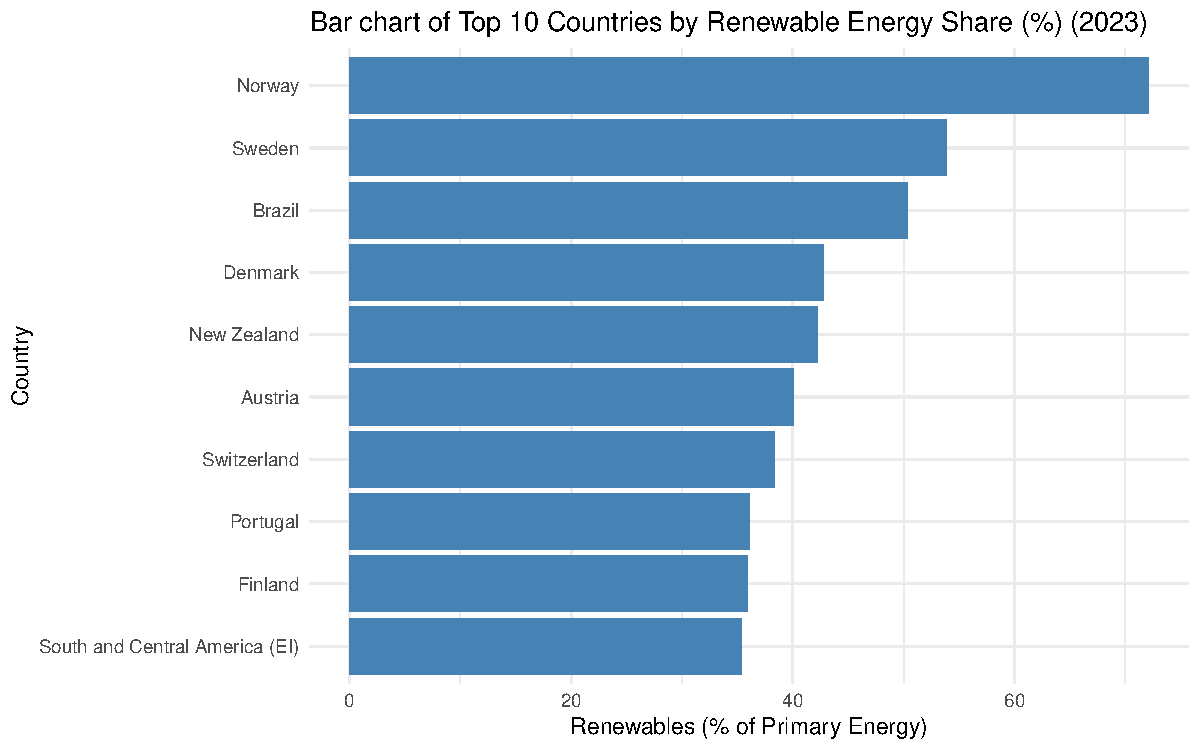
\includegraphics[keepaspectratio]{Assignment3_files/figure-pdf/fig-top10-bar-1.pdf}}

}

\caption{\label{fig-top10-bar}Bar chart of Top 10 Countries by Renewable
Energy Share (\%) (2023)}

\end{figure}%

\newpage

\hyperref[tbl-table-top10]{Table~\ref{tbl-table-top10}} and
\hyperref[fig-top10-bar]{Figure~\ref{fig-top10-bar}} present the top 10
countries with the highest renewable energy shares in 2023. Norway ranks
first with renewable share exceeding 72\%, significantly ahead of other
countries. This exceptional performance drives deeper examination of
Norway's domestic energy composition.

\newpage

\subsection{Norway: Global Leader in
2023}\label{norway-global-leader-in-2023}

To understand Norway's energy landscape, we examined its 2023
electricity mix data.

\begin{longtable}[]{@{}lr@{}}

\caption{\label{tbl-table-norway-2023}Norway's Renewable Electricity
Generation by Source in 2023 (TWh)}

\tabularnewline

\toprule\noalign{}
Source & TWh \\
\midrule\noalign{}
\endhead
\bottomrule\noalign{}
\endlastfoot
wind & 14.96 \\
hydro & 135.96 \\
solar & 0.17 \\
Other renewables including bioenergy & 0.26 \\

\end{longtable}

\begin{figure}

\centering{

\pandocbounded{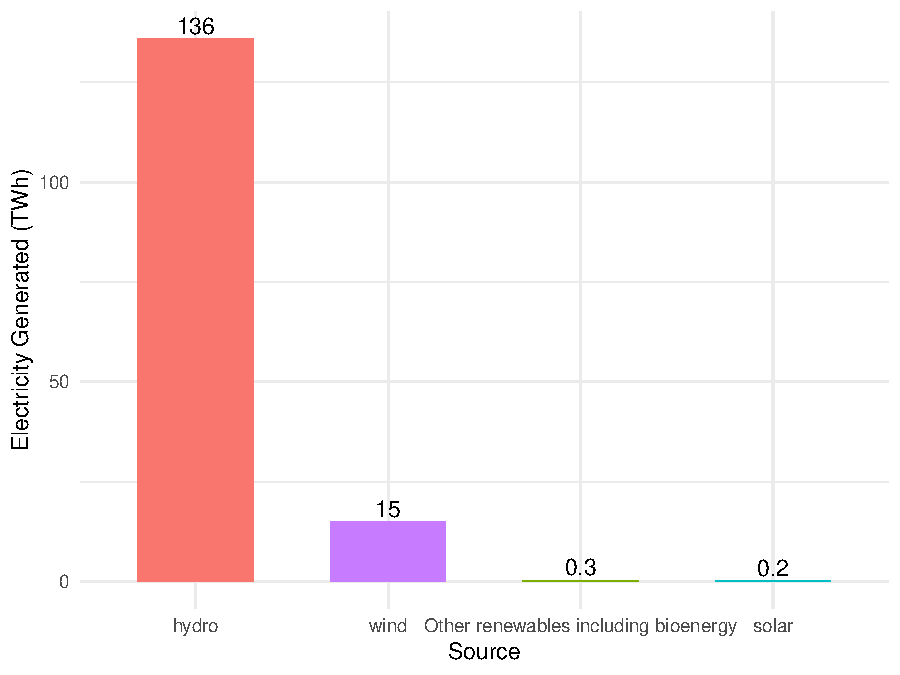
\includegraphics[keepaspectratio]{Assignment3_files/figure-pdf/fig-norway-sources-1.pdf}}

}

\caption{\label{fig-norway-sources}Norway's Renewable Electricity
Breakdown by Source in 2023 (TWh)}

\end{figure}%

\hyperref[fig-norway-sources]{Figure~\ref{fig-norway-sources}} shows
that hydropower contributed over 90\% of Norway's renewable electricity
in 2023 (136 TWh), while wind (15 TWh), solar, and bioenergy made minor
contributions.

These figures highlight that Norway's renewable energy leadership is
largely driven by its heavy reliance on \textbf{hydropower}, rather than
a diversified renewable portfolio.

\subsection{Global Hydropower Generation by Country
(2023)}\label{global-hydropower-generation-by-country-2023}

While Norway's renewable share is impressive, percentage alone may not
reflect actual capacity. A high share could result from low total energy
demand.

Therefore, we compared its absolute hydropower output with that of other
major economies to determine whether its position is based on scale, not
proportion.

\begin{figure}

\centering{

\pandocbounded{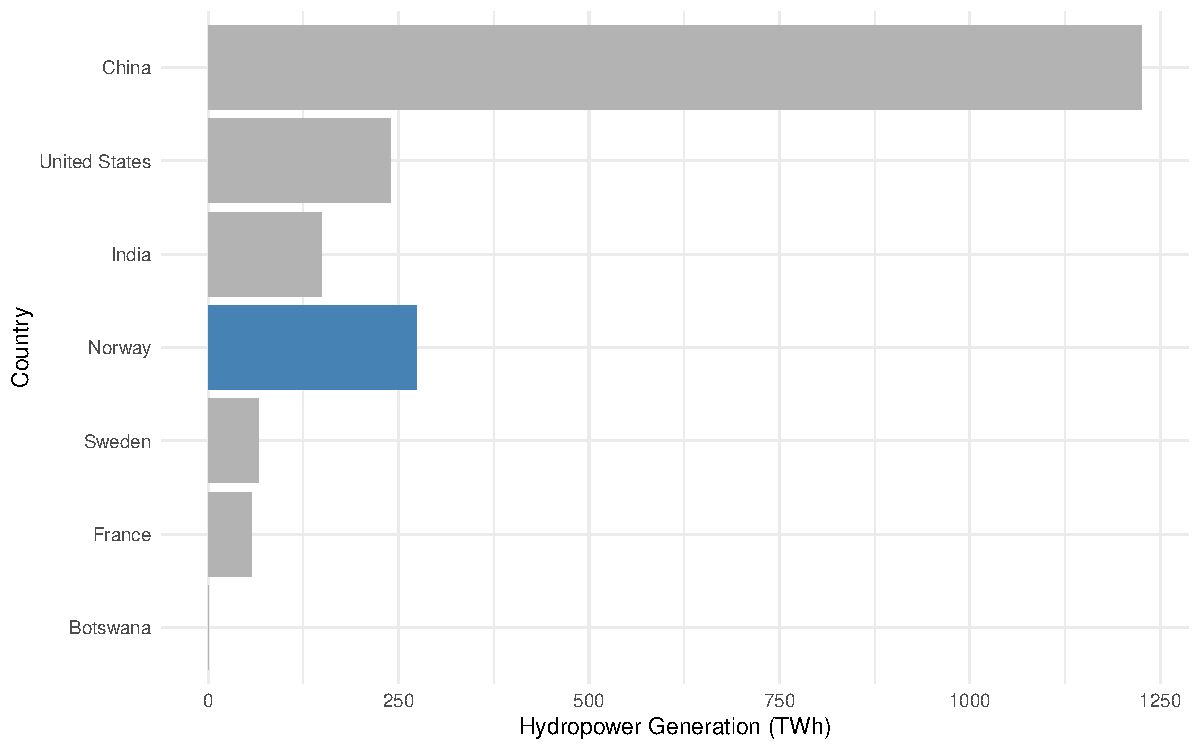
\includegraphics[keepaspectratio]{Assignment3_files/figure-pdf/fig-global-hydro-1.pdf}}

}

\caption{\label{fig-global-hydro}Global Hydropower Generation (TWh) in
2023 by Country}

\end{figure}%

\hyperref[fig-global-hydro]{Figure~\ref{fig-global-hydro}} shows
Norway's 2023 hydropower output compared to major economies. Despite its
small size, Norway produced 270 TWh, exceeding the U.S. (239 TWh) and
India (149 TWh). This comparison confirms that Norway's renewable
leadership is not only proportional, but also supported by significant
absolute generation and robust infrastructure.

\newpage

\section{Results}\label{results}

Based on the methodology outlined above, this section presents key
findings from our data analysis. In 2023, Norway led globally in
renewable energy adoption, with 72.09\% of its primary energy from
renewable sources, followed by Sweden (53.9\%) and Brazil (50.3\%)
\hyperref[tbl-table-top10]{Table~\ref{tbl-table-top10}}. These figures
highlight strong national commitments to clean energy.

\hyperref[fig-top10-bar]{Figure~\ref{fig-top10-bar}} visualizes the top
10 countries, with Norway's share standing clearly above others. This
exceptional performance reflects sustained investment and abundant
hydropower resources.

To explore the drivers of this leadership,
\hyperref[tbl-table-norway-2023]{Table~\ref{tbl-table-norway-2023}} and
\hyperref[fig-norway-sources]{Figure~\ref{fig-norway-sources}} show that
over 90\% of Norway's electricity in 2023 came from hydropower, with
limited contributions from wind, solar, and bioenergy.

\hyperref[fig-norway-trend]{Figure~\ref{fig-norway-trend}} further
illustrates that Norway has maintained a renewable share above 60\% for
two decades, signaling consistent national strategy and infrastructure
planning.

Overall, these findings suggest that Norway's leadership is not merely
proportional but supported by robust capacity. The case exemplifies how
favorable geography, long-term policy, and investment alignment can
enable sustained renewable integration at scale.

\begin{figure}

\centering{

\pandocbounded{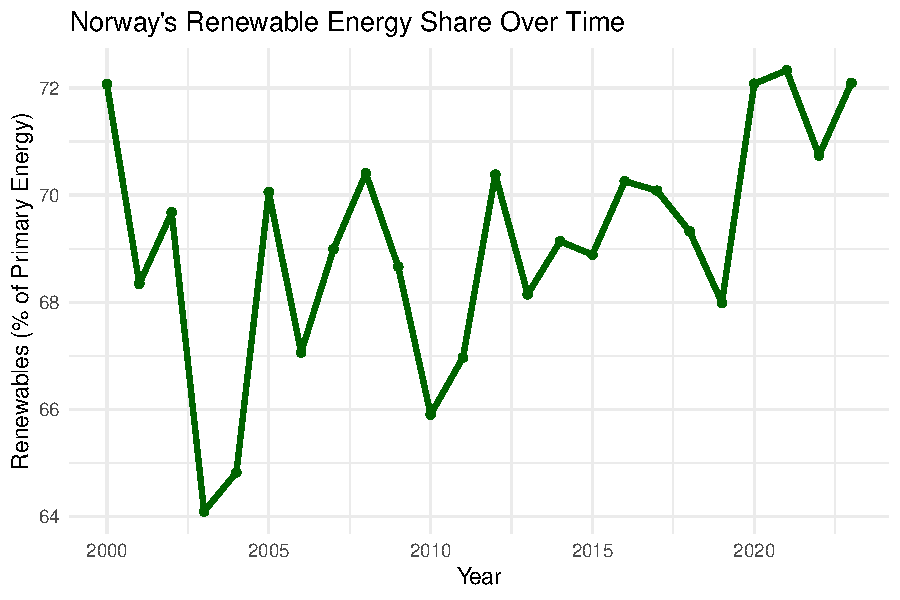
\includegraphics[keepaspectratio]{Assignment3_files/figure-pdf/fig-norway-trend-1.pdf}}

}

\caption{\label{fig-norway-trend}Norway's Renewable Energy Share
(2000--2023)}

\end{figure}%

\section{Discussion and Conclusion}\label{discussion-and-conclusion}

The findings shed light on the structural factors driving Norway's
renewable energy leadership. Its top ranking is the result of long-term
investment in hydropower, supported by favorable geography and
consistent national policy. Norway's energy profile---dominated by
hydropower---demonstrates how natural resources can be effectively
leveraged for a low-emission energy transition.

Nevertheless, dependence on a single energy source introduces potential
risks. Climate variability---such as droughts and shifting precipitation
patterns---could significantly reduce hydroelectric output.
Additionally, Norway's limited deployment of wind, solar, and bioenergy
reveals an untapped opportunity for further diversification of its
renewable portfolio.

The international comparison further reinforces that Norway's renewable
dominance is not just proportional but also absolute. This rare
combination of high renewable share and significant generation volume
underscores the success of sustained, resource-aligned energy
strategies.

In conclusion, Norway's case exemplifies how geographic advantages, when
matched with consistent national policy and infrastructure investment,
can result in world-leading performance in renewable energy integration.

A key limitation of this study is its focus on quantitative data,
without capturing differences in policy or social context. Future
research could explore how governance, incentives, and behavior shape
renewable adoption. Studying other high-performing countries may also
offer valuable policy insights.

\subsubsection{Recommendations}\label{recommendations}

\begin{itemize}
\tightlist
\item
  \emph{Diversify energy sources}: Invest in wind and solar to reduce
  over reliance on hydropower.
\item
  \emph{Modernize energy infrastructure}: Improve grid flexibility to
  integrate more variable renewables.
\item
  \emph{Export expertise}: Share Norway's policy, regulatory, and
  engineering frameworks with other nations.
\item
  \emph{Support adaptive policy}: Prepare for climate risks by
  developing redundancy and storage solutions.
\end{itemize}

\newpage

\section{References}\label{references}

\printbibliography[heading=none]





\end{document}
